\فصل{ارزیابی تجربی و تحلیل نتایج}
\label{chap:experiments}

\قسمت{دامنه و منشأ شواهد}
هدف این فصل، بررسی این پرسش است که آیا استفاده از اطلاعات خمیدگی در آموزش سریع هم‌آورد می‌تواند، با حفظ هزینهٔ کم، از بیش‌برازش فاجعه‌بار جلوگیری کند و در دادگان و معماری‌های متفاوت کارایی قابل اتکایی داشته باشد. مبنای عددی فصل، نتایج منتشرشدهٔ مقالهٔ \sora\ است \cite{sora2026}. در تدوین این پایان‌نامه آموزش تازه، جست‌وجوی ابرپارامتر تازه یا اندازه‌گیری سخت‌افزاری مستقلی انجام نشده است. بنابراین تعبیر «نتایج» در این فصل به گزارش و تحلیل آزمایش‌های مقاله اشاره دارد؛ جدول‌های بازآرایی‌شده نیز آزمایش تازه محسوب نمی‌شوند. این تفکیک برای جلوگیری از انتساب نادرست شواهد منتشرشده به اجرای مستقل پایان‌نامه ضروری است.

سه محور ارزیابی از یکدیگر جدا می‌شوند: نخست، درستی پاک و درستی زیر حمله‌های قوی؛ دوم، انتقال تنظیمات آموزش میان مسائل دسته‌بندی؛ و سوم، هزینهٔ محاسبات و رفتار شاخص هشدار \pertalign. درستی پاک به تنهایی نمی‌تواند موفقیت آموزش هم‌آورد را نشان دهد، زیرا ممکن است مدل روی نمونه‌های معمولی درست عمل کند ولی با آشفتگی کوچکی شکست بخورد. به همین ترتیب، درستی زیاد زیر همان حملهٔ تک‌گامی که در آموزش به کار رفته است، در حضور بیش‌برازش فاجعه‌بار شاهد کافی برای ستبری نیست. ازاین‌رو هر نتیجه باید همراه نام حمله، بودجه و معماری خوانده شود.

\قسمت{مدل تهدید و پروتکل ارزیابی}
در آزمایش‌های اصلی، مهاجم در فضای ورودی و با دسترسی به مدل، هزینهٔ دسته‌بندی را افزایش می‌دهد. مجموعهٔ مجاز ارزیابی در نرم $\ell_\infty$ برابر است با
\begin{equation}
 \Delta_\varepsilon(x)=\{\delta:\|\delta\|_\infty\leq\varepsilon,\quad x+\delta\in[0,1]^d\}.
 \label{eq:exp-threat}
\end{equation}
بودجه باید نسبت به مقیاس پیکسل پیش از نرمال‌سازی تفسیر شود؛ برای نمونه، $8/255$ سهمی از دامنهٔ شدت در بازهٔ $[0,1]$ است. این مدل تهدید، دستکاری محدود عددی را می‌سنجد و معادل همهٔ تغییرات طبیعی، تغییر دستگاه تصویربرداری یا حمله‌های معنایی نیست. صورت کمینه‌سازی و بیشینه‌سازی آموزش هم‌آورد و جایگاه حملهٔ چندگامی در این چارچوب در پژوهش مادری و همکاران مطرح شده است \cite{madry2018towards}.

درستی پاک سهم نمونه‌های درست دسته‌بندی‌شده بدون حمله است؛ درستی هم‌آورد سهم نمونه‌هایی است که پس از حمله نیز درست دسته‌بندی می‌شوند. \lr{FGSM} حمله‌ای تک‌گامی است و \lr{PGD-10} ده بار جهت حرکت را با استفاده از شیب به‌روزرسانی می‌کند. \lr{AutoAttack}، با اختصار \lr{AA}، ارزیابی ترکیبی قوی‌تری فراهم می‌کند که وابستگی نتیجه به تنظیم یک حملهٔ منفرد را کاهش می‌دهد \cite{croce2020reliable}. ترکیب استاندارد آن شامل \lr{APGD-CE}، \lr{APGD-DLR}، \lr{FAB} و \lr{Square Attack} است و حمله‌های مبتنی بر شیب و جست‌وجوی بدون شیب را کنار هم قرار می‌دهد. این توضیح دربارهٔ چارچوب مرجع است؛ مقالهٔ \sora\ نسخه و تمام جزئیات پیکربندی ارزیابی را در متن چاپی مشخص نمی‌کند. هیچ‌یک از این سنجه‌های تجربی گواهی ریاضی ستبری نیستند. همچنین عدد \lr{PGD-10} را نمی‌توان به جای عدد \lr{AA} گذاشت یا اختلاف آن‌ها را صرفاً نوسان تصادفی نامید.

مقاله در صفحهٔ ۸ بودجهٔ پیش‌فرض را $8/255$ اعلام می‌کند، اما پیوست \lr{D} در صفحهٔ ۳۱ برای تصاویر خاکستری \lr{TissueMNIST} بودجه را به $3/255$ کاهش می‌دهد تا تغییرات تصویری بیش از اندازه نشوند. شکل ۱۲ در صفحهٔ ۳۹ نیز سقف گام متناسب با این استثنا را نمایش می‌دهد. در این فصل استثنای پیوست صریحاً حفظ شده است. این اعداد به معنای نامحسوس‌بودن اثبات‌شدهٔ آشفتگی برای همهٔ بیماران یا همهٔ انواع تصویر نیستند؛ چنین ادعایی به ارزیابی تخصصی مستقل نیاز دارد.

\قسمت{دادگان، معماری‌ها و تنظیمات آموزش}
\زیرقسمت{تنوع مسائل دسته‌بندی}
جدول \ref{tab:exp-datasets} ابعاد و اندازهٔ مجموعه‌های مورد استفاده را نشان می‌دهد. \lr{CIFAR-10} و \lr{CIFAR-100} به دلیل اندازهٔ کوچک تصاویر و رواج در مطالعات آموزش سریع، نقطهٔ شروع مناسبی هستند \cite{krizhevsky2009learning}. افزایش شمار کلاس‌ها در \lr{CIFAR-100} و افزایش وضوح و تنوع در \lr{TinyImageNet} امکان بررسی دشواری‌هایی را فراهم می‌کند که در مسئلهٔ ده‌کلاسه آشکار نمی‌شوند. \lr{ImageNet-100} نیز گسترش آزمایش به تصاویر $224\times224$ را می‌آزماید، ولی نمونه‌ای از کل \lr{ImageNet} است و نباید به عنوان ارزیابی هزارکلاسه معرفی شود.

% Provenance: published SORA paper, Table 3 p.30 and Appendix D pp.31--33; newly compiled presentation, not an original thesis experiment or seminar table.
\begin{table}[tbp]
\centering
\caption[دادگان، ابعاد ورودی و بودجه ارزیابی]{ویژگی دادگان بر اساس جدول ۳ و پیوست \lr{D} مقاله، صفحات ۳۰ تا ۳۳ \cite{sora2026}. ستون بودجه از توضیح صفحهٔ ۳۱ افزوده شده است؛ جدول بازتدوین‌شده از مقاله است.}
\label{tab:exp-datasets}
\begin{latin}
\small
\setlength{\tabcolsep}{4pt}
\begin{tabular}{lrrrrr}
\hline
\rl{دادگان} & \rl{ابعاد ورودی} & \rl{دسته‌ها} & \rl{آموزش} & \rl{آزمون} & $\varepsilon$ \\
\hline
CIFAR-10 & $3\times32\times32$ & 10 & 50,000 & 10,000 & $8/255$ \\
CIFAR-100 & $3\times32\times32$ & 100 & 50,000 & 10,000 & $8/255$ \\
TinyImageNet & $3\times64\times64$ & 200 & 100,000 & 10,000 & $8/255$ \\
ImageNet-100 & $3\times224\times224$ & 100 & 117,000 & 5,000 & $8/255$ \\
PathMNIST & $3\times28\times28$ & 9 & 89,996 & 7,180 & $8/255$ \\
TissueMNIST & $1\times28\times28$ & 8 & 165,466 & 47,280 & $3/255$ \\
\hline
\end{tabular}
\end{latin}
\end{table}

دو مجموعهٔ پزشکی از \lr{MedMNIST} انتخاب شده‌اند \cite{yang2023medmnist}. \lr{PathMNIST} شامل تصاویر بافت‌شناسی رنگی مرتبط با دسته‌بندی بافت در سرطان روده و \lr{TissueMNIST} شامل تصاویر خاکستری سلول‌های قشر کلیه است. مقاله برای اولی ۱۰٬۰۰۴ نمونهٔ اعتبارسنجی و برای دومی ۲۳٬۶۴۰ نمونهٔ اعتبارسنجی نیز ذکر می‌کند. اختلاف دامنهٔ این تصاویر با تصاویر طبیعی، آزمایش انتقال تنظیمات را معنادار می‌سازد. منظور از تعمیم در اینجا، عمدتاً توانایی یک روش آموزش با تنظیمات ثابت برای آموزش مدل‌های جداگانه روی مسائل مختلف است؛ مدل آموزش‌دیده روی \lr{CIFAR} مستقیماً روی بافت پزشکی آزموده نشده است.

مطابق شکل ۸ مقاله، توزیع کلاس‌ها در دادگان طبیعی متوازن‌تر است، درحالی‌که دو دادگان پزشکی نامتوازن‌اند و این وضعیت در \lr{TissueMNIST} شدیدتر است. بافت ریز و شباهت بیشتر میان کلاس‌ها نیز در تفسیر نویسندگان از دشواری آموزش نقش دارد. بااین‌حال آزمایش عاملی مستقلی که اثر عدم توازن را از اثر بافت جدا کند گزارش نشده است. بنابراین نسبت‌دادن تمام افت ستبری به یکی از این عوامل، از شواهد موجود فراتر می‌رود. درستی کلی نیز جای سنجه‌های هر کلاس یا تحلیل خطاهای بالینی را نمی‌گیرد.

\زیرقسمت{تنظیمات مشترک و تفاوت‌های ضروری}
چهار معماری اصلی عبارت‌اند از \lr{PreActResNet-18}، \lr{ResNet-18}، \lr{WideResNet-28-10} و \lr{SENet-18}. این انتخاب به ترتیب امکان مقایسهٔ پیش‌فعال‌سازی، اتصال باقیمانده، افزایش عرض و توجه کانالی را فراهم می‌کند \cite{he2016identity,he2016deep,zagoruyko2016wide,hu2018squeeze}. اشتراک خانوادگی برخی از این شبکه‌ها سبب می‌شود تنوع معماری را کامل ندانیم. آزمایش‌های \lr{ViT-Small} در صفحات ۵۷ و ۵۸ مقاله تکمیلی‌اند و به علت مقیاس محدود دادگان و نبود آزمایش پیش‌آموزش بزرگ، جای ارزیابی فراگیر مبدل‌های بینایی را نمی‌گیرند.

بهینه‌ساز اصلی \lr{SGD} با تکانهٔ $0.9$ و افت وزن $5\times10^{-4}$ است. برای دادگان طبیعی، برنامهٔ چرخه‌ای نرخ یادگیری از $0.01$ تا $0.2$ و سپس بازگشت به $0.01$ گزارش شده است. برای دو دادگان پزشکی، کاهش کسینوسی از $0.05$ تا حداقل $10^{-3}$ به کار می‌رود. در \lr{CIFAR} حاشیه‌گذاری چهارپیکسلی، برش تصادفی و بازتاب افقی؛ در \lr{TinyImageNet} حاشیه‌گذاری هشت‌پیکسلی؛ و در دادگان پزشکی چرخش تصادفی ده‌درجه‌ای و بازتاب افقی ذکر شده است. پس «تنظیم ثابت» به معنای یکسان‌بودن همهٔ جزئیات آماده‌سازی دادگان نیست.

ابرپارامترهای اصلی \sora\ برابر $\alpha_0=0.02$، $\beta=0.05$ و $\alpha_{\max}=2\varepsilon$ هستند. بر اساس صفحات ۷ و ۳۵، در بخش عمدهٔ آموزش \lr{CIFAR} سقف گام انتخاب می‌شود، ولی در \lr{PathMNIST} نیاز به کاهش گام بیشتر است. این رفتار با انگیزهٔ سازگارکردن حمله با هندسهٔ هزینه سازگار است؛ به خودی خود اثبات نمی‌کند که برآورد خمیدگی در هر دسته دقیق است. جزئیات وقفه در انتقال اطلاعات میان دسته‌ها، تفاوت \pertalign\ با ضریب کنترل گام و محدودیت مشخصات بازتولید در پیوست \ref{chap:technical-appendix} آمده‌اند.

\زیرقسمت{مقایسهٔ منصفانه و معنای تنظیم ثابت}
خطوط مبنا از روش‌های سادهٔ \lr{FGSM} و \lr{FGSM-RS} تا روش‌های دارای منظم‌سازی، چندشروعی یا گام سازگار را دربرمی‌گیرند. \lr{PGD-2}، \lr{PGD-10} و \lr{TRADES} نیز مراجع چندگامی‌اند. هدف اصلی مقایسه، بررسی کارایی عملی آموزش سریع است که در آن هزینهٔ جست‌وجوی مکرر ابرپارامترها نیز اهمیت دارد \cite{wong2020fast}. بااین‌حال باید میان هزینهٔ یک اجرای آموزش و هزینهٔ کل انتخاب تنظیمات تمایز گذاشت؛ مقاله برای هزینهٔ کل جست‌وجوی همهٔ روش‌ها زمان عددی جامعی ارائه نمی‌کند.

پیوست \lr{M.3}، صفحهٔ ۶۰، توضیح می‌دهد که تنظیمات پیشنهادی مقالات مبنا استفاده و در مسائل جدید اصلاحات مستدل اعمال شده‌اند. جست‌وجوی عمده به \lr{CIFAR-10/100} و دو معماری متداول محدود بوده و آزمایش‌های محدودی روی \lr{PathMNIST} نیز برای \sora\ و خطوط مبنا انجام شده است. سپس پارامترهای روش برای ارزیابی‌های دیگر ثابت شده‌اند. بنابراین تعبیر دقیق، استفاده از یک مجموعهٔ نهایی مشترک پس از تنظیم محدود است؛ تعبیر «روش بدون هیچ تنظیمی ساخته شده است» درست نیست. از سوی دیگر، این پروتکل پاسخ مسئلهٔ انتقال تنظیمات را می‌دهد و الزاماً بهترین نتیجهٔ ممکن هر روش پس از جست‌وجوی نامحدود را نمی‌سنجد.

\قسمت{نتایج اصلی روی دو مسئلهٔ دشوار}
جدول \ref{tab:exp-main} اعداد جدول ۱ مقاله را با همان معیارها بازنویسی می‌کند. در \lr{PathMNIST}، \sora\ به درستی پاک $85.93$ و درستی \lr{AA} برابر $32.91$ درصد می‌رسد. اختلاف با \lr{N-FGSM} در معیار \lr{AA} برابر $31.26$ واحد درصد و با \lr{AAER} برابر $30.43$ واحد درصد است. این اختلاف‌ها واحد درصد هستند؛ بیان آن‌ها به صورت درصد رشد نسبی معنای متفاوتی دارد. روی \lr{ImageNet-100} نیز مقدار \lr{AA} از $15.52$ برای \lr{N-FGSM} و $17.18$ برای \lr{AAER} به $18.56$ درصد برای \sora\ افزایش یافته است.

% Provenance: published SORA paper, main Table 1 p.9, epsilon=8/255; exact original entries, not seminar results and not a new run.
\begin{table}[tbp]
\centering
\caption[نتایج اصلی روی دادگان بافت‌شناسی و صدکلاسه]{نتایج اصلی \lr{PreActResNet-18} با $\varepsilon=8/255$؛ بازنویسی جدول ۱ مقاله، صفحهٔ ۹ \cite{sora2026}. همهٔ مقادیر درصدند.}
\label{tab:exp-main}
\begin{latin}
\begin{tabular}{lrrrr}
\hline
& \multicolumn{2}{c}{PathMNIST} & \multicolumn{2}{c}{ImageNet-100} \\
\rl{روش} & \rl{پاک} & AA & \rl{پاک} & AA \\
\hline
FGSM & 46.06 & 0.42 & 15.94 & 0.00 \\
N-FGSM & 74.89 & 1.65 & 49.40 & 15.52 \\
AAER & 83.54 & 2.48 & 48.26 & 17.18 \\
SORA & 85.93 & 32.91 & 57.26 & 18.56 \\
\hline
\end{tabular}
\end{latin}
\end{table}

در این دو مسئله، بهبود ستبری در گزارش اصلی با افت درستی پاک همراه نشده است. این نکته نشان می‌دهد که در این مقایسه، ستبری مدل صرفاً با محدودکردن شدید ظرفیت یا قربانی‌کردن درستی پاک حاصل نشده است. بااین‌حال صفحهٔ ۵۹ تصریح می‌کند که آزمایش \lr{ImageNet-100} به دلیل هزینهٔ زیاد تنها یک اجرا داشته است. از این گزارش نمی‌توان پراکندگی میان بذرها، فاصلهٔ اطمینان یا معناداری آماری اختلاف $1.38$ واحد درصدی با \lr{AAER} را استنتاج کرد. برای سایر آزمایش‌ها سه بذر گزارش شده، اما این امر عدم قطعیت نتیجهٔ تک‌اجرایی را برطرف نمی‌کند.

گزارش اصلی را باید از نتایج تجمیعی پیوست جدا نگه داشت. برای نمونه، جدول ۳۲ صفحهٔ ۵۳ برای \sora\ روی همان نام دادگان و معماری، پاک $84.88\pm0.99$ و \lr{AA} برابر $35.54\pm1.55$ می‌دهد. متن مقاله رابطهٔ دقیق این مقادیر با پاک $85.93$ و \lr{AA} برابر $32.91$ در جدول ۱ را روشن نمی‌کند. این فصل هر دو گزارش را با منشأ مستقل حفظ می‌کند؛ نه میانگین‌گیری تازه انجام می‌دهد و نه یکی را اصلاح عدد دیگر معرفی می‌کند. تشخیص نقش بذر، ایست بازرسی یا تنظیم دقیق به فرادادهٔ اجرای اصلی نیاز دارد.

\قسمت{خوانش تفصیلی نتایج و حدود تعمیم}
شکل \ref{fig:exp-generalization} نمای کلی مقاله را نشان می‌دهد. در هر مسئله، درستی هر روش بر بیشترین درستی همان مسئله تقسیم شده است؛ بنابراین عدد نزدیک یک نشانهٔ نزدیکی به بهترین نتیجهٔ آن ستون است. این نمایش برای یافتن شکست‌های بزرگ مفید است، ولی مقادیر مطلق و اندازهٔ اختلاف‌های کوچک را پنهان می‌کند. همچنین بیشترین درستی پاک و بیشترین درستی هم‌آورد ممکن است متعلق به دو روش متفاوت باشند. ازاین‌رو نباید دو میلهٔ نسبی را به عنوان دو ویژگی یک مدل ایده‌آل مشترک تفسیر کرد.

% Provenance: published SORA paper, Figure 6 p.8 (normalization explained p.47); supplied paper crop, not seminar artwork and not newly measured data.
\begin{figure}[tbp]
\centering
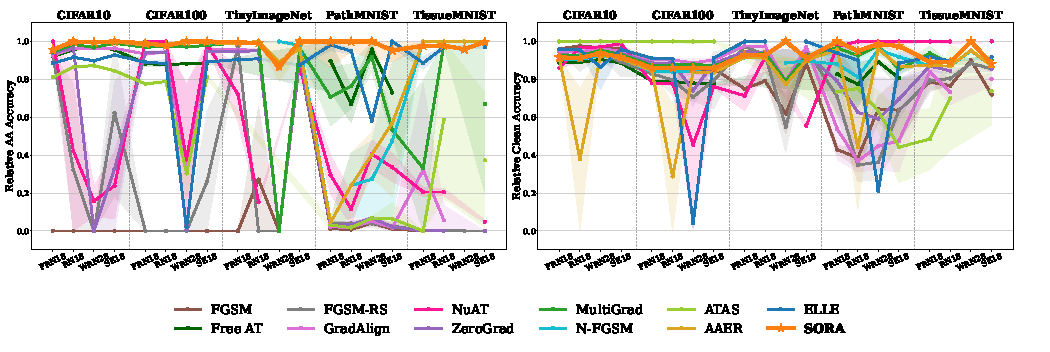
\includegraphics[width=\textwidth]{images/paper_generalization.pdf}
\caption[تعمیم تنظیمات میان دادگان و معماری‌ها]{تعمیم تنظیمات میان دادگان و معماری‌ها؛ بازنشر شکل ۶ مقاله، صفحهٔ ۸ \cite{sora2026}. درستی \lr{AA} و پاک نسبت به بهترین مقدار هر مسئله نرمال شده‌اند؛ جزئیات نرمال‌سازی در صفحهٔ ۴۷ مقاله آمده است.}
\label{fig:exp-generalization}
\end{figure}

جدول \ref{tab:exp-natural} نمونه‌هایی از نتایج مطلق را برای \lr{PreActResNet-18} کنار هم می‌آورد. روی \lr{CIFAR-10}، درستی \lr{AA} روش \sora\ برابر $43.83$ درصد است؛ \lr{N-FGSM} و \lr{AAER} به ترتیب $43.95$ و $43.96$ درصد دارند و \lr{NuAT} به $45.90$ درصد می‌رسد، اما درستی پاک آن کمتر است. در \lr{CIFAR-100} نیز $21.56$ درصد \sora\ بیشترین مقدار جدول نیست. این اعداد از یک مبادلهٔ عملی میان پاک، ستبر و هزینه پشتیبانی می‌کنند، ولی گزارهٔ برتری مطلق در همهٔ ستون‌ها را تأیید نمی‌کنند.

% Provenance: published SORA paper, selected rows of Tables 20 p.48, 24 p.50, 28 p.52; newly compiled cross-dataset table, not an original paper table or seminar result. Central values only; published +/- omitted explicitly in caption.
\begin{table}[tbp]
\centering
\caption[گزیده نتایج مطلق روی دادگان تصویری طبیعی]{گزیدهٔ درستی‌های گزارش‌شده برای \lr{PreActResNet-18}، از جدول‌های ۲۰، ۲۴ و ۲۸ مقاله در صفحات ۴۸، ۵۰ و ۵۲ \cite{sora2026}. این چینش تازه از مقاله فقط مقادیر مرکزی را نشان می‌دهد؛ مؤلفه‌های $\pm$ منبع برای اختصار حذف شده‌اند.}
\label{tab:exp-natural}
\begin{latin}
\small
\begin{tabular}{llrrr}
\hline
\rl{دادگان} & \rl{روش} & \rl{پاک} & PGD-10 & AA \\
\hline
CIFAR-10 & FGSM-RS & 82.61 & 47.16 & 42.48 \\
& NuAT & 75.09 & 50.28 & 45.90 \\
& N-FGSM & 79.05 & 48.73 & 43.95 \\
& AAER & 79.38 & 48.59 & 43.96 \\
& SORA & 79.90 & 48.64 & 43.83 \\
& PGD-10 & 79.37 & 50.60 & 46.15 \\
\hline
CIFAR-100 & FGSM-RS & 52.70 & 0.00 & 0.00 \\
& NuAT & 49.66 & 27.81 & 22.13 \\
& N-FGSM & 53.43 & 26.25 & 21.75 \\
& SORA & 54.74 & 26.12 & 21.56 \\
& PGD-10 & 53.57 & 27.64 & 22.88 \\
\hline
TinyImageNet & FGSM-RS & 47.46 & 19.67 & 14.95 \\
& N-FGSM & 44.66 & 20.18 & 15.77 \\
& AAER & 44.72 & 19.94 & 15.71 \\
& SORA & 45.30 & 20.07 & 15.38 \\
\hline
\end{tabular}
\end{latin}
\end{table}

اهمیت تفکیک حمله‌ها در نمونهٔ \lr{FGSM-RS} روی \lr{CIFAR-100} روشن است: جدول ۲۴ درستی \lr{FGSM} را $55.02$ درصد گزارش می‌کند، درحالی‌که \lr{PGD-10} و \lr{AA} هر دو صفرند. چنین فاصله‌ای نمونهٔ بارز شکست ارزیابی تک‌گامی است. در مقابل، برای \sora\ نیز \lr{PGD-10} بزرگ‌تر از \lr{AA} است؛ این اختلاف یادآوری می‌کند که جلوگیری از فروپاشی کامل، هم‌معنای حل مسئلهٔ ستبری در برابر همهٔ حمله‌ها نیست. شدت ارزیابی باید همراه نتیجه باقی بماند.

جدول \ref{tab:exp-architecture} مواردی را نشان می‌دهد که تغییر معماری رتبه‌بندی را عوض می‌کند. در \lr{TinyImageNet/WideResNet}، درستی پاک \sora\ بیشتر ولی \lr{AA} آن کمتر از \lr{N-FGSM} است. در \lr{PathMNIST/SENet}، \lr{ELLE} درستی \lr{AA} بیشتری دارد، اما درستی پاک آن کمتر است. در \lr{TissueMNIST} نیز بعضی خطوط مبنا از نظر \lr{AA} اندکی بهترند. حفظ این موارد در گزارش از انتخاب گزینشی نتایج جلوگیری می‌کند و مفهوم تعمیم را به پایداری قابل قبول در مجموعه‌ای از مسائل محدود می‌سازد، نه بردن تک‌تک مقایسه‌ها.

% Provenance: published SORA paper, Tables 26 p.51, 30 p.53, 35--36 p.55, 38 p.56; selected exact central entries newly compiled here, not seminar data. Tissue budget follows Appendix D p.31.
\begin{table}[tbp]
\centering
\caption[وابستگی نتایج به معماری و دادگان]{نمونه‌های وابستگی نتیجه به معماری؛ چینش تازه از جدول‌های ۲۶، ۳۰، ۳۵، ۳۶ و ۳۸ مقاله، صفحات ۵۱، ۵۳، ۵۵ و ۵۶ \cite{sora2026}. فقط مقادیر مرکزی درصدی آمده‌اند؛ بودجهٔ \lr{TissueMNIST} مطابق صفحهٔ ۳۱ برابر $3/255$ است.}
\label{tab:exp-architecture}
\begin{latin}
\small
\begin{tabular}{lllrrr}
\hline
\rl{دادگان} & \rl{معماری} & \rl{روش} & \rl{پاک} & PGD-10 & AA \\
\hline
CIFAR-100 & WRN-28 & N-FGSM & 57.28 & 27.82 & 23.74 \\
& WRN-28 & SORA & 58.58 & 27.93 & 23.77 \\
TinyImageNet & WRN-28 & N-FGSM & 48.47 & 21.21 & 16.58 \\
& WRN-28 & SORA & 54.59 & 18.73 & 14.31 \\
PathMNIST & SENet-18 & ELLE & 76.45 & 44.10 & 39.88 \\
& SENet-18 & SORA & 85.32 & 41.21 & 34.76 \\
TissueMNIST & PreAct-18 & N-FGSM & 57.47 & 49.25 & 48.15 \\
& PreAct-18 & SORA & 58.86 & 48.55 & 47.06 \\
TissueMNIST & WRN-28 & AAER & 57.83 & 50.00 & 48.95 \\
& WRN-28 & SORA & 60.68 & 47.91 & 45.92 \\
\hline
\end{tabular}
\end{latin}
\end{table}

برای سنجش فاصله با آموزش چندگامی، جدول \ref{tab:exp-path-extended} مفید است. در گزارش تجمیعی \lr{PathMNIST}، \sora\ با درستی پاک $84.88$ از \lr{PGD-10} با $77.62$ بالاتر است، ولی \lr{AA} آن $35.54$ در برابر $50.70$ درصد است. بنابراین انتخاب روش به اولویت کاربرد بستگی دارد: اگر بیشترین ستبری تجربی هدف اصلی باشد و هزینه محدودیت نباشد، آموزش چندگامی همچنان گزینهٔ جدی است. متن محدودیت‌های مقاله نیز همین مرز را در صفحهٔ ۵۹ می‌پذیرد.

% Provenance: published SORA paper, Table 32 p.53; exact selected entries including published +/-; separate aggregate report from main Table 1 and ablation Table 2, not seminar and not new measurements.
\begin{table}[tbp]
\centering
\caption[مقایسه تفصیلی با روش‌های چندگامی روی دادگان بافت‌شناسی]{گزارش تفصیلی مستقل \lr{PathMNIST/PreActResNet-18} از جدول ۳۲ مقاله، صفحهٔ ۵۳ \cite{sora2026}. علامت $\pm$ عیناً از منبع نقل شده و در این پایان‌نامه فاصلهٔ اطمینان تازه‌ای محاسبه نشده است.}
\label{tab:exp-path-extended}
\begin{latin}
\small
\begin{tabular}{lrrr}
\hline
\rl{روش} & \rl{پاک} & PGD-10 & AA \\
\hline
N-FGSM & $74.86\pm6.14$ & $18.84\pm4.14$ & $1.90\pm0.77$ \\
ELLE & $79.80\pm6.67$ & $40.52\pm2.38$ & $34.60\pm1.05$ \\
SORA & $84.88\pm0.99$ & $43.56\pm1.66$ & $35.54\pm1.55$ \\
PGD-2 & $83.49\pm0.34$ & $47.50\pm0.51$ & $40.84\pm0.23$ \\
PGD-10 & $77.62\pm1.45$ & $54.47\pm0.89$ & $50.70\pm0.53$ \\
TRADES & $75.25\pm0.73$ & $51.94\pm0.88$ & $48.28\pm0.74$ \\
\hline
\end{tabular}
\end{latin}
\end{table}

\قسمت{حذف مؤلفه‌ها و حساسیت ابرپارامترها}
\زیرقسمت{سهم سازگاری و تنوع آشفتگی}
جدول \ref{tab:exp-ablation} دقیقاً به آزمایش حذف مؤلفه‌های جدول ۲ مقاله تعلق دارد. مقدار پایهٔ پاک $84.69$ است و ارزیابی ستبری با \lr{PGD-10} انجام شده است. این آزمایش را نباید ادامهٔ همان اجرای جدول \ref{tab:exp-main} دانست که پاک $85.93$ و معیار \lr{AA} دارد. نام مشترک روش و معماری برای یکسان‌انگاشتن تنظیمات یا ایست بازرسی کافی نیست. در اینجا تفسیر اختلاف‌ها تنها درون خود جدول حذف مؤلفه‌ها انجام می‌شود.

% Provenance: published SORA paper, main Table 2 p.9, PathMNIST/PreActResNet-18 component ablation; exact values, not main Table 1, not seminar or a new experiment.
\begin{table}[tbp]
\centering
\caption[آزمایش حذف مؤلفه‌های روش پیشنهادی]{حذف مؤلفه‌ها در \lr{PathMNIST}؛ جدول ۲ مقاله، صفحهٔ ۹ \cite{sora2026}. این گزارش \lr{PGD-10} با پاک پایهٔ $84.69$ مستقل از جدول اصلی \lr{AA} است.}
\label{tab:exp-ablation}
\begin{latin}
\small
\begin{tabular}{lrrr}
\hline
\rl{تنظیم} & \rl{پاک} & FGSM & PGD-10 \\
\hline
SORA (\rl{پایه}) & 84.69 & 57.51 & 45.56 \\
\rl{بدون نمونه‌گیری تصادفی} & 85.67 & 58.89 & 45.35 \\
\rl{برش اندازه گام} & 86.82 & 52.02 & 34.08 \\
\rl{بدون گام تطبیقی} & 89.93 & 28.30 & 17.23 \\
\hline
\end{tabular}
\end{latin}
\end{table}

حذف انتخاب گام بهینه، درستی \lr{PGD-10} را از $45.56$ به $17.23$ درصد می‌رساند، درحالی‌که درستی پاک افزایش می‌یابد. این نتیجه با نقش گام سازگار در جلوگیری از تولید نمونه‌های آموزشی ضعیف سازگار است. محدودکردن گام در گونهٔ موسوم به \lr{Clamping Step-Size} نیز مقدار را به $34.08$ کاهش می‌دهد. در مقابل، حذف نمونه‌گیری تصادفی تنها افت $0.21$ واحد درصدی دارد. چون جدول پراکندگی یا تکرارهای این مقایسه را مشخص نمی‌کند، این اختلاف کوچک به تنهایی شاهد معناداری آماری نقش نمونه‌گیری نیست؛ اثر بزرگ‌تر سازگاری گام پشتوانهٔ عددی روشن‌تری دارد.

\زیرقسمت{حساسیت به سقف و ضریب گام}
جدول \ref{tab:exp-hyper} برش‌های مشخصی از جست‌وجوی ابرپارامترهای پیوست \lr{F} را ارائه می‌کند. افزایش $\alpha_{\max}$ در \lr{CIFAR-10} با $\beta=0.05$ و $\alpha_0=0.02$، درستی \lr{PGD-10} را از $45.70$ به $49.36$ درصد افزایش می‌دهد، اما پاک را از $83.97$ به $75.87$ کاهش می‌دهد. بنابراین انتخاب $2\varepsilon$ صرفاً انتخاب بیشترین عدد ستبری نیست و مصالحهٔ میان دو معیار را منعکس می‌کند. روی \lr{PathMNIST}، تغییر $\alpha_0$ اثر شدیدتری دارد؛ این امر با فعال‌شدن بیشتر سازوکار سازگار در آن دادگان سازگار است.

% Provenance: published SORA paper, Tables 5--10 pp.35--36; newly compiled selected hyperparameter slices, exact central values; not an original table, seminar evidence, or new sweep.
\begin{table}[tbp]
\centering
\caption[حساسیت به ابرپارامترهای کنترل گام]{برش‌های جست‌وجوی ابرپارامتر \sora؛ چینش تازه از جدول‌های ۵ تا ۱۰ مقاله، صفحات ۳۵ و ۳۶ \cite{sora2026}. هر سطر یک تنظیم گزارش‌شده است و معیار ستبری \lr{PGD-10} است.}
\label{tab:exp-hyper}
\begin{latin}
\small
\begin{tabular}{lrrrrr}
\hline
\rl{دادگان} & $\beta$ & $\alpha_0$ & $\alpha_{\max}/\varepsilon$ & \rl{پاک} & PGD-10 \\
\hline
CIFAR-10 & 0.05 & 0.02 & 1.5 & 83.97 & 45.70 \\
CIFAR-10 & 0.05 & 0.02 & 2.0 & 79.84 & 48.70 \\
CIFAR-10 & 0.05 & 0.02 & 2.5 & 75.87 & 49.36 \\
CIFAR-100 & 0.05 & 0.02 & 1.5 & 58.41 & 24.63 \\
CIFAR-100 & 0.05 & 0.02 & 2.0 & 54.06 & 26.29 \\
CIFAR-100 & 0.05 & 0.02 & 2.5 & 50.98 & 27.05 \\
PathMNIST & 0.05 & 0.01 & 2.0 & 85.06 & 44.01 \\
PathMNIST & 0.05 & 0.02 & 2.0 & 84.69 & 45.56 \\
PathMNIST & 0.05 & 0.05 & 2.0 & 90.42 & 19.90 \\
PathMNIST & 0.02 & 0.02 & 2.0 & 87.26 & 35.84 \\
PathMNIST & 0.10 & 0.02 & 2.0 & 84.94 & 44.47 \\
\hline
\end{tabular}
\end{latin}
\end{table}

نمونهٔ $\alpha_0=0.05$ روی \lr{PathMNIST} مهم است: پاک $90.42$ همراه با \lr{PGD-10} برابر $19.90$ گزارش می‌شود. بنابراین ثابت‌ماندن مجموعهٔ نهایی پارامترها نباید با بی‌حساسیتی روش به همهٔ مقادیر اشتباه شود. شواهد نشان می‌دهند یک تنظیم مشترک مفید وجود دارد، اما پیرامون آن نواحی ضعیف نیز دیده می‌شوند. علاوه بر این، انتخاب نهایی بخشی از شواهد همان مطالعه است؛ ارزیابی روی مسائل واقعاً تازه برای آزمودن دامنهٔ انتقال ضروری خواهد بود.

\قسمت{بودجهٔ آشفتگی و اندازهٔ دسته}
جدول \ref{tab:exp-budget} نتایج تغییر بودجهٔ آموزش در \lr{CIFAR-10} را نقل می‌کند. در بودجهٔ $4/255$، \sora\ هم پاک و هم \lr{PGD-10} بیشتری از \lr{N-FGSM} دارد؛ اما در $16/255$، درستی \lr{PGD-10} آن $27.12$ در برابر $29.23$ درصد است. بنابراین نتیجهٔ دقیق این است که روش از فروپاشی کامل در بودجه‌های گزارش‌شده دور مانده، نه اینکه همیشه بیشترین ستبری را دارد. کاهش درستی پاک با افزایش بودجه نیز نشان می‌دهد مقایسهٔ روش‌ها در بودجه‌های متفاوت بدون ذکر محدودیت حمله گمراه‌کننده است.

% Provenance: published SORA paper, Table 11 p.36; selected exact central values, newly compiled clean/PGD-10 pairs; not seminar or new training. These are training-budget experiments, distinct from Table 12 test-budget evaluation.
\begin{table}[tbp]
\centering
\caption[حساسیت روش‌ها به بودجه آموزش]{حساسیت به بودجهٔ آموزش در \lr{CIFAR-10}، از جدول ۱۱ مقاله، صفحهٔ ۳۶ \cite{sora2026}. هر خانه به ترتیب پاک و \lr{PGD-10} است؛ فقط مقادیر مرکزی منبع نقل شده‌اند.}
\label{tab:exp-budget}
\begin{latin}
\small
\begin{tabular}{lrrrr}
\hline
\rl{روش} & $4/255$ & $8/255$ & $12/255$ & $16/255$ \\
\hline
ATAS & 90.63 / 61.53 & 87.25 / 41.91 & 86.89 / 12.08 & 83.89 / 8.86 \\
N-FGSM & 87.40 / 66.44 & 79.05 / 48.73 & 69.36 / 37.54 & 61.20 / 29.23 \\
SORA & 87.85 / 66.86 & 79.90 / 48.64 & 72.18 / 37.32 & 67.66 / 27.12 \\
\hline
\end{tabular}
\end{latin}
\end{table}

تغییر بودجه در زمان آزمون پرسش دیگری است: در جدول ۱۲ صفحهٔ ۳۷، برای \sora\ مقادیر \lr{PGD} در بودجه‌های $3/255$، $5/255$، $9/255$، $13/255$ و $17/255$ به ترتیب $68.97$، $62.72$، $43.97$، $28.45$ و $14.17$ درصدند. در بودجهٔ کوچک نخست، \lr{ATAS} با $74.26$ بالاتر است و در بودجهٔ آخر \lr{N-FGSM} با $14.21$ اندکی بالاتر قرار می‌گیرد. عنوان ستون منبع در این جدول \lr{PGD} است؛ تعداد گام را از جدول‌های دیگر به آن تحمیل نمی‌کنیم. این داده‌ها نباید با آزمایش آموزش مدل‌های جداگانه در بودجه‌های متفاوت ادغام شوند.

پیوست \lr{F.1}، صفحهٔ ۳۵، حساسیت اندازهٔ دسته را نیز گزارش می‌کند. برای \sora{}، افزایش اندازه از ۳۲ به ۱۲۸، پاک را از $74.74$ به $79.90$ و \lr{PGD-10} را از $46.38$ به $48.64$ درصد می‌رساند؛ در اندازهٔ ۵۱۲ این دو مقدار $79.86$ و $47.00$ هستند. پس بزرگ‌ترکردن دسته تضمین بهبود یکنواخت نیست. این آزمایش برای روشی که اطلاعات دستهٔ قبلی را به کار می‌برد اهمیت دارد، زیرا تغییر اندازهٔ دسته هم نوسان تخمین و هم شمار به‌روزرسانی‌ها را عوض می‌کند. داده‌های موجود اثر مستقل این دو عامل را جدا نمی‌کنند.

\قسمت{کارایی محاسباتی و حافظه}
شکل \ref{fig:exp-efficiency} اندازه‌گیری مقاله روی \lr{PathMNIST/PreActResNet-18} را نشان می‌دهد. مبنای زمانی، آموزش ۳۰ دوره روی \lr{NVIDIA GeForce RTX 4090} است و محور عمودی درستی \lr{PGD-10} را نمایش می‌دهد. طبق صفحهٔ ۵۹، زمان حلقهٔ اصلی آموزش سنجیده شده و ذخیره و بارگذاری ایست‌های بازرسی کنار گذاشته شده‌اند. تکرار اندازه‌گیری زمان و کنترل تداخل فرایندها نیز توسط نویسندگان گزارش شده است. بااین‌حال مقدار دقیق زمان هر روش، تعداد تکرارها و پراکندگی عددی آن‌ها در جدول چاپی ارائه نشده‌اند؛ این فصل از خواندن تقریبی نقاط نمودار برای ساختن زمان دقیق خودداری می‌کند.

% Provenance: published SORA paper, Figure 7 p.8, measurement protocol p.59; supplied paper crop, not seminar figure or thesis hardware measurements.
\begin{figure}[tbp]
\centering
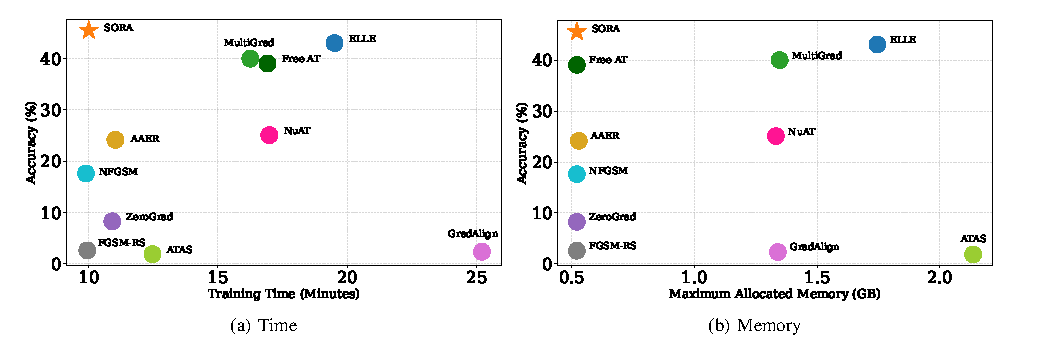
\includegraphics[width=\textwidth]{images/paper_efficiency.pdf}
\caption[بده‌بستان زمان، حافظه و درستی هم‌آورد]{زمان آموزش و بیشینهٔ حافظهٔ تخصیص‌یافته در برابر درستی \lr{PGD-10}؛ بازنشر شکل ۷ مقاله، صفحهٔ ۸ \cite{sora2026}. تنظیم: \lr{PathMNIST}، \lr{PreActResNet-18}، ۳۰ دوره و \lr{RTX 4090}. این اندازه‌گیری متعلق به مقاله است.}
\label{fig:exp-efficiency}
\end{figure}

دادهٔ شمارش گذرها، برخلاف مختصات نمودار زمان، به صورت عددی در جدول ۱۹ صفحهٔ ۴۸ موجود است. \sora\ به دو گذر پیشرو و دو گذر پسرو در هر دسته نیاز دارد؛ \lr{PGD-10} یازده گذر از هر نوع و \lr{TRADES} دوازده گذر پیشرو و یازده گذر پسرو دارد. این شمارش دلیل ساختاری کم‌هزینه‌بودن روش را توضیح می‌دهد، اما نسبت $11/2$ را نمی‌توان نسبت شتاب واقعی نامید: اندازهٔ گراف، اندازهٔ دسته و استفاده از حافظه بر زمان مؤثرند. جدول دقیق شمارش و استثنای بازپخش \lr{Free AT} در پیوست آمده است.

قید حافظه نیز بخشی از نتیجه است. صفحهٔ ۴۷ مقاله گزارش می‌کند که نیاز حافظهٔ \lr{ATAS} مانع اجرای آن روی \lr{TinyImageNet} با سخت‌افزار موجود شده است. نبود سطر یک روش در جدول به معنای صفر بودن درستی آن نیست. همچنین ناپایداری عددی \lr{ELLE} در بعضی تنظیمات \lr{WideResNet}، طبق صفحهٔ ۴۸، باید از بیش‌برازش فاجعه‌بار متمایز شود. هر دو ممکن است نتیجهٔ نامطلوب بسازند، اما سازوکار شکست و راه اصلاح یکسانی ندارند.

\قسمت{اعتبار شاخص هشدار و زمان پیش‌آگاهی}
شواهد \pertalign\ در صفحات ۴۴ تا ۴۶ مقاله، روند چند سنجه را با مسیر آموزش مقایسه می‌کنند. در نمونهٔ مشخص \lr{FGSM}، افت \pertalign\ و \lr{GradAlign} حدود دستهٔ ۳۷۷۵ آغاز می‌شود، درحالی‌که جدایی آشکار درستی \lr{FGSM} و \lr{PGD} حدود دستهٔ ۳۸۲۵ دیده می‌شود. بنابراین این نمونه تقریباً ۵۰ دسته پیش‌آگاهی دارد. این اختلاف یک مشاهدهٔ نموداری در یک مسیر مشخص است؛ نه میانگین زمان هشدار برای همهٔ اجراها و نه تضمین یک مهلت ثابت پیش از هر فروپاشی است.

پیوست \lr{J.1} توضیح می‌دهد که \lr{ELLE} نیز پس از انتقال و مقیاس‌بندی لگاریتم می‌تواند در همان حوالی واکنش نشان دهد، هرچند اوج آن دیرتر است و محاسبهٔ سنجه هزینهٔ بیشتری دارد. در نتیجه، مزیت اصلی \pertalign\ ترکیب واکنش زودهنگام با استفادهٔ مجدد از شیب‌های موجود است، نه ادعای اینکه هیچ سنجهٔ دیگری زود واکنش نمی‌دهد. نرخ نمونه‌های هم‌آورد نامتعارف و واگرایی خروجی‌ها در مثال مقاله دیرتر تغییر می‌کنند. این تفاوت ترتیب زمانی با فرض تغییر هندسهٔ هزینه پیش از افت آشکار درستی سازگار است.

شکل ۱۵ مقاله همراهی افت شاخص و افت ستبری را در چند ترکیب دادگان، معماری و روش نشان می‌دهد و حتی نمونهٔ افت، بازیابی و افت دوباره دارد. بااین‌حال مقاله نرخ هشدار کاذب، حساسیت آماری، آستانهٔ ازپیش‌تعیین‌شده یا توزیع زمان پیش‌آگاهی را به صورت عددی گزارش نمی‌کند. ازاین‌رو نمی‌توان \pertalign\ را احتمال کالیبره‌شدهٔ وقوع بیش‌برازش دانست. برای استفادهٔ عملی به عنوان سامانهٔ هشدار، تعریف رویداد، انتخاب آستانه روی اعتبارسنجی و آزمون مستقل آن لازم است؛ این‌ها در این پایان‌نامه اجرا نشده‌اند.

\قسمت{برداشت نهایی از شواهد}
مجموع نتایج از سودمندی سازگاری گام برای جلوگیری از شکست‌های بزرگ آموزش سریع پشتیبانی می‌کند، به‌ویژه در \lr{PathMNIST} که بسیاری از خطوط مبنا با تنظیمات متداول ستبری اندکی دارند. آزمایش حذف مؤلفه‌ها نیز نقش انتخاب گام را روشن‌تر از اثر کوچک حذف نمونه‌گیری نشان می‌دهد. بااین‌حال درستی \lr{AA} در برخی مسائل برای خطوط مبنا بیشتر است و آموزش چندگامی روی مسئلهٔ دشوار پزشکی فاصلهٔ قابل توجهی دارد. نتیجهٔ مناسب، مصالحهٔ مطلوب و انتقال‌پذیری تنظیم نهایی در دامنهٔ آزموده‌شده است.

محدودیت‌های شواهد شامل تک‌اجرایی‌بودن \lr{ImageNet-100}، پوشش ناقص برخی ترکیب‌ها بر اثر حافظه، مشخص‌نبودن همهٔ جزئیات ارزیابی در متن مقاله و تفاوت چند گزارش عددی میان متن و پیوست است. این موارد با افزودن رقم، فرض‌کردن تنظیمات رایج یا ساختن فاصلهٔ اطمینان حل نمی‌شوند. پیوست فنی، نگاشت ادعاها به صفحات منبع و مشخصات لازم برای بازتولید آینده را ثبت می‌کند تا مرز میان دادهٔ منتشرشده، محاسبهٔ ساده از آن داده و پیشنهاد ارزیابی آینده روشن بماند.
